\section{Introduction}
\label{sec:intro}

%Human interaction with computers is one of the most fundamental components in today's complex systems, and interfaces are crucial for such interactions. In a traditional setting, a user accesses a computer or host system, most commonly a PC to configure remote end systems such as a web server. These web servers can host a range of applications and provide a web-based user interface (UI) that the user uses to communicate with the end services. Figure~\ref{fig:motivation} illustrates four such application interfaces such as critical infrastructures, automation systems, financial transaction, and many more day to day services. All such applications rely on human input and proper understanding of output from the server. Hence, the correctness of the input and output is of uttermost importance. And most of these systems are hosted remotely and provide a web-based UI. 
Web-based interfaces are very prevalent to remotely configure safety-critical systems such as remote PLC, medical device, and many security-sensitive applications such as financial transactions etc. The high complexity of modern operating systems, softwares and hardware components has proven that computer systems largely remain vulnerable to attacks. A compromised computer threatens the integrity and the confidentiality of any interaction between the user and a remote server. It can easily alter the data exchanged between the user and the remote server, trick the user to perform unintended actions, or observe any sensitive IO data. E.g., a compromised browser can manipulate the input parameters to remote safety-critical end-systems such as critical infrastructures, automation systems, financial transaction, and many more day to day services.

Recent introduction of trusted computing architectures like Intel's SGX has enabled secure computations and secure data storage on otherwise untrusted computing platforms. However, such architectures do not directly enable secure user interaction. Additionally, the recently discovered microarchitectural attacks have shown that enclaved execution environments, like the one provided by SGX, can be compromised as well.

\iffalse
\begin{figure}[t]
\centering
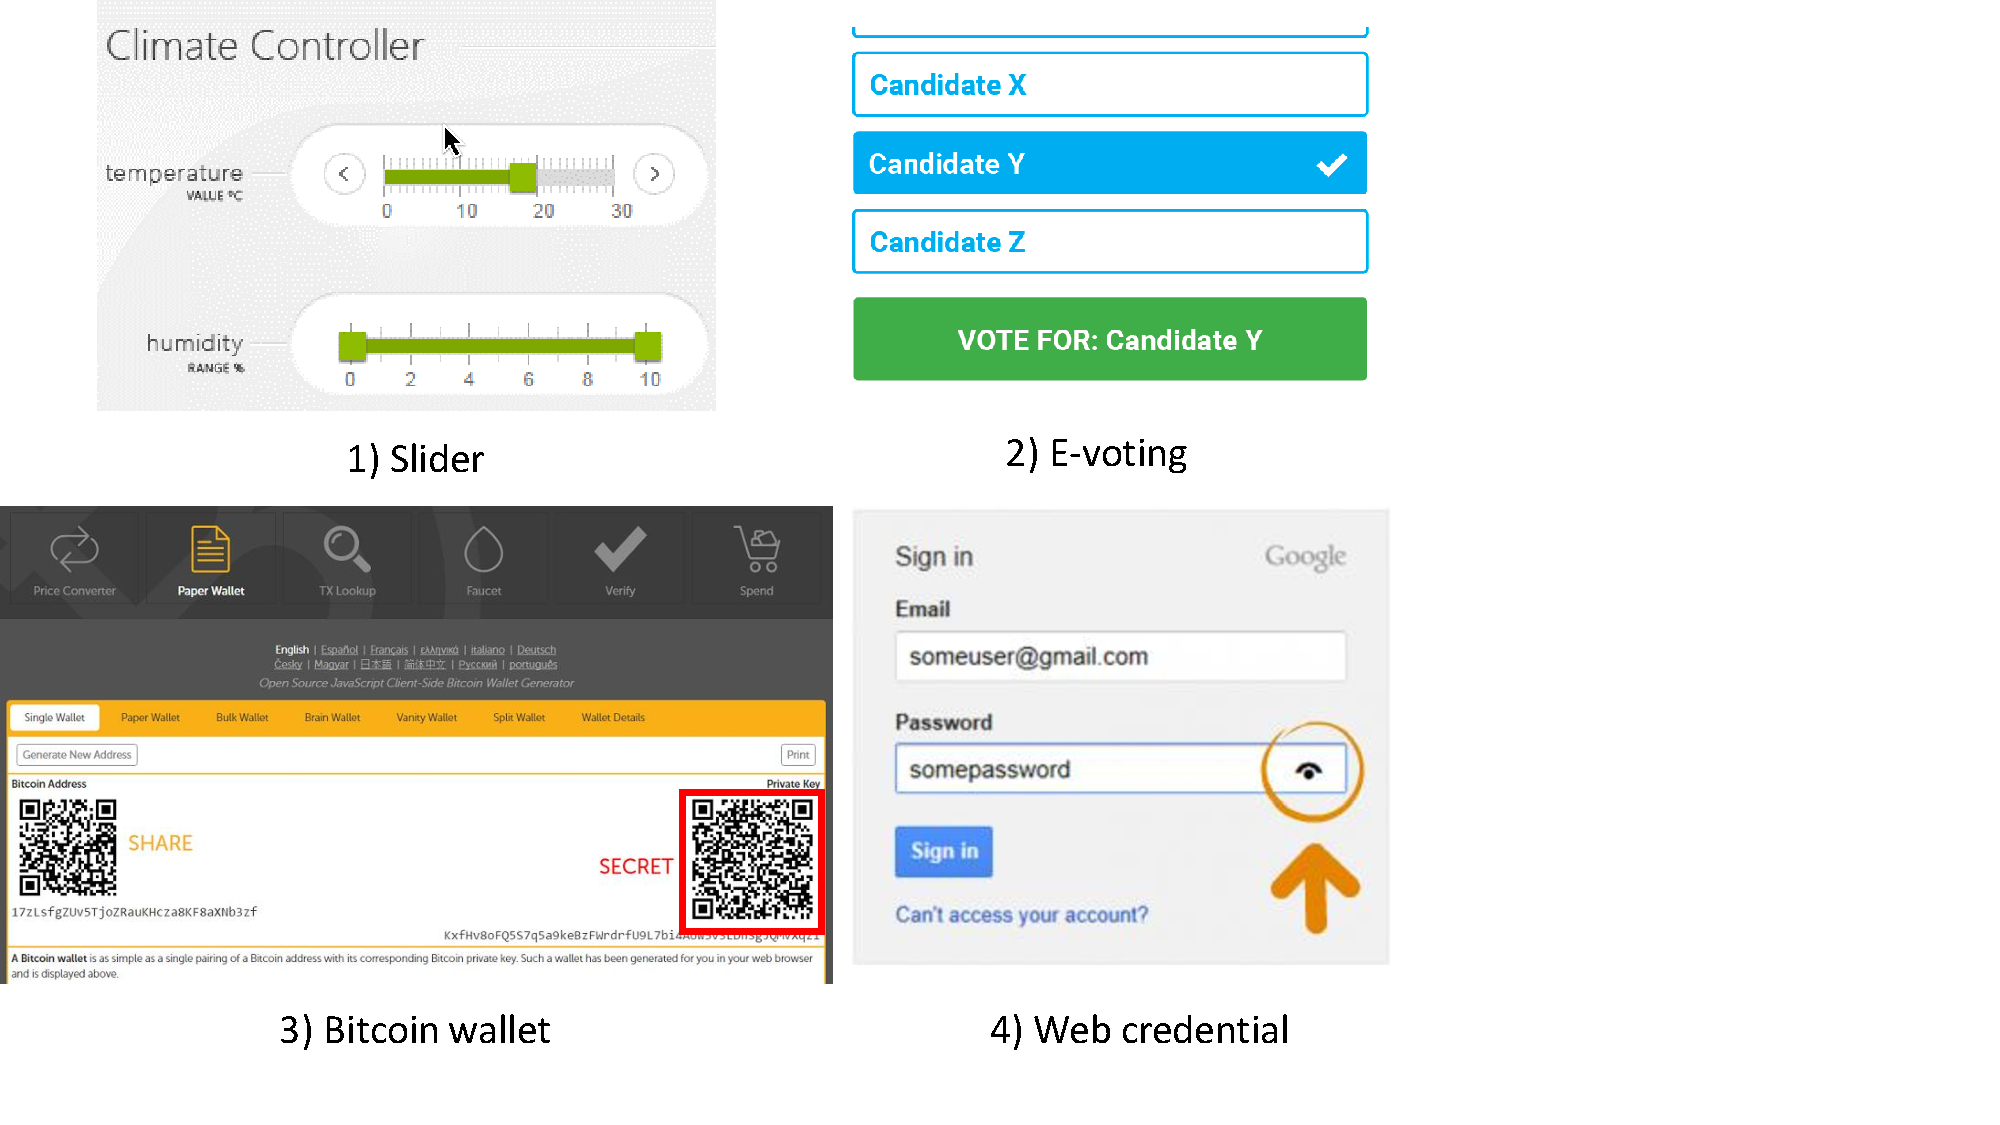
\includegraphics[trim={0 1cm 10cm 0}, clip, width=\linewidth]{motivation.pdf}
\caption{\textbf{Motivating examples.} 1) Pointer based UI elements that sets parameters to remote safety-critical device, 2) E-voting where the voting privacy and integrity is critical, 3) Financial transactions such as bitcoin wallet that shows sensitive information such as the user's private key and 4) web applications that provide an option for the user to reveal credentials.}
\spacesave
\label{fig:motivation}
\centering
\end{figure}
\fi


IO operation between the user and a remote server in the presence of an untrusted host is a long-standing problem. \emph{Trusted path} provides a secure channel between the user (HID) and the end-point which is typically a trustworthy application running on the host. Trusted path ensures that user inputs reach the intended application unmodified, and all the outputs presented to the user are generated by the legitimate application. Trusted path to the local host is a well-researched area where many solutions focus on using trusted software components such as a trusted hypervisor. In work done by Zhou et al.~\cite{zhou2012building}, the authors proposed a generic trusted path on $x86$ systems with a pure hypervisor-based design. SGXIO~\cite{weiser2017sgxio} employed both the hypervisor and trusted execution environment (TEE) such as Intel SGX. Hypervisors require a large TCB, hard to deploy and are often impractical in real world scenarios as most of the existing verified hypervisors offer very limited set of features. TEEs such as SGX relies on OS the mediate IO and also is vulnerable to microarchitectural attacks~\cite{van2018foreshadow}.

%However, when considering an untrusted host, trusted path to the local host does not provide any advantage. 
%In such an attacker model, it is crucial to ensure a trusted path from the user to a trusted remote server. 
Remote trusted path variant is non-trivial as typically all the IO operations are mediated by the operating system, device drivers, etc. All these mediator are attacker-controlled when an  untrusted host is considered. To solve this problem, solutions typically rely on trusted external devices. Transaction confirmation devices~\cite{filyanov2011uni,weigold2011secure} allow the user to review her input data on a trusted device that is physically separated from the untrusted host but suffers from poor usability and is only limited to simple inputs. Bump in the Ether~\cite{McCPerRei2006} and IntegriKey~\cite{IntegriKey} use external embedded devices to sign input parameters. However, such solutions do not support output integrity; hence, the attacker can execute UI manipulation attacks to trick the user into providing incorrect inputs.

%Out of the numerous works, Fidelius~\cite{Fidelius} provides the most comprehensive solution to protect keyboard inputs from a compromised browser using external devices and a \js interpreter that runs inside an SGX enclave. Fidelius maintains overlays on display, specifically on the input text boxes to hide sensitive user inputs from the browser. Fidelius relies on the user monitoring continuously LED lights and information on an overlaid bar to provide its integrity and confidentiality properties. Several research works~\cite{egelman2008you,sobey2008exploring} show that in the real-world, passive security indicators do not provide adequate security, and suffer from user habituation. Furthermore, the output integrity such as the integrity of the UI layout and the labels could be easily broken. For example, the attacker can change instructions on the screen to influence the user by changing the unit of an input value to a safety-critical device. The attacker can even trick the user into putting additional information that may compromise the integrity of the input data. Not supporting mouse also exposes Fidelius to early form submission and clickjacking attack. The host can emulate a mouse click on the submit button while the user in in the process of typing into the text field. Causing an early form submission with incomplete input - violation of input integrity. Fidelius is also vulnerable to clickjacking~\cite{huang2012clickjacking} attack where the attacker could trick the user into putting incorrect data into the sensitive text field by making the user following a wrong mouse pointer. Fidelius is also vulnerable to  microarchitectural attacks on SGX enclaves~\cite{van2018foreshadow} that extract attestation keys, relay attacks~\cite{dhar2018proximitee} that relay all user data to the attacker's platform, etc. From the functional point of view, Fidelius only supports keyboard inputs and text box as input UI. We discuss such drawbacks in details along with some of the relevant solutions in Section~\ref{sec:problemStatement:existingSolution}.

Out of the numerous works, Fidelius~\cite{Fidelius} provides the most comprehensive solution to protect keyboard inputs from a compromised browser using external devices and a \js interpreter that runs inside an SGX enclave. Fidelius maintains overlays on display, specifically on the input text boxes to hide sensitive user inputs from the browser. Fidelius relies on the user monitoring continuously LED lights and information on an overlaid bar to provide its integrity and confidentiality properties. Several research works~\cite{egelman2008you,sobey2008exploring} show that in the real-world, passive security indicators do not provide adequate security, and suffer from user habituation. Furthermore, the attacker can manipulate labels of the UI elements to trick the user into providing incorrect input. Not supporting mouse also exposes Fidelius to early form submission attack where the host can emulate a mouse click on the submit button while the user in in the process of typing into the text field. Causing an early form submission with incomplete input - violation of input integrity. Fidelius is also vulnerable to  microarchitectural attacks on SGX enclaves~\cite{van2018foreshadow} that extract attestation keys, relay attacks~\cite{dhar2018proximitee} that relay all user data to the attacker's platform, etc. From the functional point of view, Fidelius only supports keyboard inputs and text box as input UI. We discuss such drawbacks in details along with some of the relevant solutions in Section~\ref{sec:problemStatement:existingSolution}. 
 
 
\myparagraph{Our contribution} The shortcomings of the previous works provide the groundwork of our paper \name that provides IO integrity and confidentiality guarantee without introducing major changes to the existing systems and user interaction, and is generic across all the IO devices and majority of the frequently used complex user interactions. \name is build on the idea that i) input integrity is not achievable without both input and output integrity are ensured simultaneously, and ii) all the input modalities are needed to be protected as they influence each other. \name uses a trusted low-TCB auxiliary device that we call \device which works as a generic IO hub between all user IO devices and the untrusted host. \device does not have any explicit network capability to communicate with the trusted remote server. Instead, the \device uses the host as an untrusted transport. 

\name ensures output integrity and confidentiality by sending an encoded UI to the host that only the \device can overlay on a small part of the screen. The overlay is possible as the \device intercepts the display signal between the host and the monitor. The overlay generated by the \device ensures that the host can neither observe nor manipulate any output information; hence, it can not trick the user. \device supports a subset of HTML5 UI elements that are frequently used in the majority of web applications. The \device also isolated the overlaid part of the screen by dimming out the rest when the user moves the mouse pointer on the overlaid UI. By doing so, \name aids the user to be more attentive to the security-critical UI on the screen. \name requires minor modification in the user interactions and \name's active way to distinguish the trusted UI on the screen does not risk user habituation. The \device analyzes the intercepted HDMI frames to understand the correct user context, such as if the user moves her mouse over a specific UI element and clicks there. On top of the mouse pointer, the \device overlays another pointer that is clearly visible to the user. In this way \name mitigates clickjacking attacks. The \device also intercepts the mouse and keyboard signals and match them with the display signal that is received from the untrusted host. If both the input and output co-relates, the \device signs all the input and sends them to the remote server. The signed input from the \device ensures input integrity and authenticity. \device is a fully plug-and-play device that is compatible with any host system regardless of their architecture or OS and does not require the user to install any software on the host. Note that our realization of \name uses an external device. However, the current system architecture can be modified, e.g., \device can be integrated into the graphics processor. We now summarize the contributions of \name as: 

%In our design of \name, the \device acts as the \emph{root-of-trust} as the mere fact of connecting all the IO devices to the \device ensures the IO security. 


\begin{mybullet}
  \item The drawbacks in the existing research work provide the understanding that without securing both output and input integrity simultaneously, none of the two can be achieved (refer to Section~\ref{sec:approach}). In our knowledge, \name is the first paper that provides such a concrete understanding. The paper also provide a formal security analysis.
  \item We describe the design of \name, a system that provides a remote trusted path from the server to the user, in an attacker-controlled environment. The design of \name leverages a small, low-TCB auxiliary device that acts as a \emph{root-of-trust} for the IO. \name protects the integrity and confidentiality of the UI, specifically the integrity and confidentiality of mouse pointer and keyboard input. \name is further designed to avoid user habituation. Unlike transaction confirmation devices, \name can be used to protect complex IO interaction that are common in today's web forms with rich and complex UI elements e.g., radio-button, drop-down menu etc. (refer to Section~\ref{sec:systemDesign} \&~\ref{sec:confidentiality}).
  %\item We analyze the security of our solution in depth and argue why \name achieves IO integrity. We also discuss potential side channel leakages that may undermine the confidentiality of IO (refer to Section~\ref{sec:securityAnalysis}). 
  \item We also implement a prototype of \name (that includes \device and \name \js) that is practical and easy to use (refer to Section~\ref{sec:prototype} \&~\ref{sec:eval}).
\end{mybullet}


\myparagraph{Organization of the paper} The organization of this paper is as the following. Section~\ref{sec:problemStatement} provides the detailed motivation, problem statement, state-of-the-art and the goals of this paper. Section~\ref{sec:approach} provides the system \& attacker model, challenges and a brief overview of our solution. We discussed the technical details of \name in Section~\ref{sec:systemDesign}. Section~\ref{sec:securityAnalysis} provides in-depth security analysis of \name. Section~\ref{sec:prototype} and~\ref{sec:eval} provide details of \name prototype implementation and corresponding evaluation. Finally, Section~\ref{sec:relatedWorks} and~\ref{sec:conclusion} provides the related research works and concludes the paper respectively.

%%%%%%%%%%%%%%%%%%%%%%%%%%%%%%%%%%%%%%
     %\myparagraph{State of the art} A trusted path provides roughly provide a set of four security properties to the communication channel between the user and the end system. Ensuring that the user performs intended actions to the remote server, typically, requires to assure that the user gets authentic output from the server. \emph{Output integrity} ensures that the information from the server reaches to the user in the intended form. For example, a user configuring a safety-critical device remotely bases her inputs in the current state of the system. As illustrated in the Figure~\ref{fig:motivation}, a compromised host could trick the user into performing unintended actions by providing incorrect feedback about the actual status. \emph{Output confidentiality} enables applications that require that the trusted paths offer a mechanism for the remote server to show secret information to the user. Figure~\ref{fig:motivation} illustrates such cases when a web server delivers a private key of a crypto-wallet to the user which should be kept hidden to the untrusted host.

%Once that output security is achieved, the trusted paths should guarantee that the remote servers accept only inputs generated by the honest user - \emph{Input integrity}. This feature is critical for the integrity of user actions in case of a compromised host. As shown in Figure~\ref{fig:motivation}, the user submits her inputs, and the remote server assures that a malicious host has not altered the user's original inputs. \emph{Input confidentiality} provides stricter security guarantees. Other applications (e.g., e-voting) require a higher level of security, the inputs should be sent to the server as generated by the user---input integrity---and preferably the host should not have access to inputs. Note that, to provide input security, trusted paths should guarantee at first output security.


%Trusted path is in focus in several recent research works. Several ways could be employed to realize the trusted path. For example, Filyanov et. al~\cite{filyanov2011uni} proposed transaction confirmation device that requires the user to use a separate device to confirm the input parameters. This allows the user to review her input data on a separate trusted device that is physically separated from the untrusted host. Trusted execution environments (TEE) such as Intel SGX, ARM TrustZone, TPM, Intel TXT, etc. provide isolated code execution, and can be used to achieve trusted path. Previous research works such as Intel SGX and trusted hypervisor-based SGXIO~\cite{weiser2017sgxio}, Intel SGX based ProximiTEE~\cite{dhar2018proximitee}, TPM and TXT based trusted path~\cite{filyanov2011uni}, and ARM TrustZone based trusted path~\cite{sun2015trustotp} are the example of trusted path construction based on TEEs. All of these solutions require specialized platforms with processors that support such infrastructure. VButton~\cite{li2018vbutton} uses ARM TrustZone to overlay buttons on the mobile devices that confirm if the user taps on a specific button. Processor-TEE such as Intel SGX primarily provides execution privacy and code integrity. In most of the cases, IO is still mediated by the OS. InContext~\cite{huang2012clickjacking} presents different clickjacking attacks variants and their solution by ensuring context (both temporal and visual) and pointer integrity in the trusted browser setting. Trusted hypervisors and secure micro-kernels are also choices for contrasting Trusted path. Sel4~\cite{klein2009sel4} is a functional hypervisor that is formally verified and has a kernel size of only $8400$ lines of code. In work done by Zhou et al.~\cite{zhou2012building}, the authors proposed a generic trusted path on $x86$ systems in pure hypervisor-based design. Examples of other hypervisor-based works can be found in systems such as Overshadow~\cite{Overshadow}, Virtual ghost~\cite{criswell2014virtual}, Inktag~\cite{hofmann2013inktag}, TrustVisor~\cite{mccune2010trustvisor}, Splitting interfaces~\cite{ta2006splitting}, $SP^3$~\cite{yang2008using}, etc.

%In spite of numerous existing research works on trusted path, none of the existing system provides an end-to-end secure trusted path that works on generic input devices, handles complex UI and user interactions, and introduces minimal or no changes to the existing systems and user's behaviour. This leads to the realization of our proposed solution, \name.


 